\subsection{\textit{\textbf{Algoritmo DaC}}}


\subsubsection{Árbol de recursión}
Podemos analizar el tiempo de ejecución construyendo el árbol de recursión para el algoritmo. Definamos $k=max(longitud(s_1), longitud(s_2))$, de modo que $k$ representa la longitud de la cadena más larga ingresada al algoritmo. Debido a que en cada llamada a la función se decrementa una de las dos cadenas, podemos intuir que la altura máxima del árbol será igual a $k$. En cada llamada al algoritmo se ejecutan tres llamadas recursivas, por lo que cada nodo del árbol tendrá tres ramas. Esto continuará hasta que se alcance el caso base, es decir, cuando la longitud de alguna de las cadenas sea $0$.

\begin{center}
\fbox{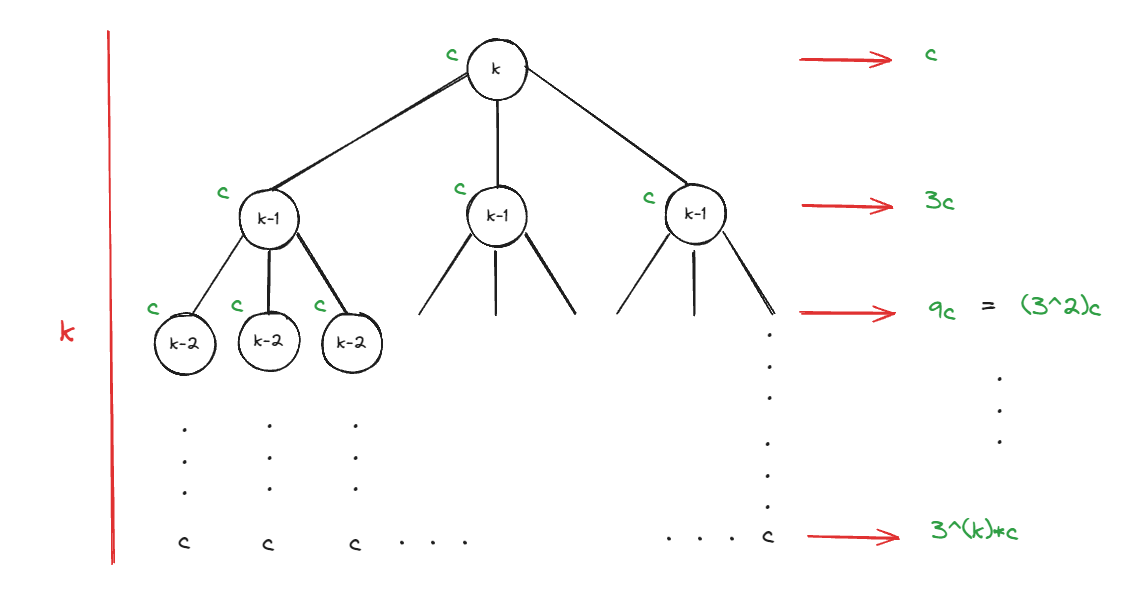
\includegraphics[width=15cm, height=7.5cm,]{images/arbol_recursion_dac.png}}\\
\vspace{0.02in}
\small\textcolor{FSBlue}{Imagen 1: Árbol de recursión del algoritmo \textit{Edit Distance}} con enfoque Divide and Conquer.
\end{center}

Utilizando el \quotes{ancho} ($3^kc$) del árbol podemos obtener una buena aproximación para una cota superior del tiempo de ejecución del algoritmo. Podemos probarlo si asumimos que el tiempo de ejecución del algoritmo está dado por la siguiente ecuación de recurrencia:

\[T(k)=3T(k-1)+k\]

Podemos probar que nuestro aproximación es válida sustituyendo esta desigualdad $T(k) \leq c \cdot 3^k$ en el término recursivo de la ecuación de recurrencia que definimos anteriormente:
\begin{align*}
T(k) &= 3T(k-1)+k \\
T(k) &\leq 3(c \cdot 3^{k-1})+k \\
T(k) &\leq c \cdot 3^k+k
\end{align*}

Si aplicamos notación \textit{Big-O} al lado derecho de la desigualdad resultante obtenemos $O(3^k)$, recordando que $k=max(longitud(s_1), longitud(s_2))$.


\subsubsection{Análisis por partes}
Para realizar el análisis asintótico del algoritmo de distancia de edición utilizando el enfoque de Divide and Conquer, primero debemos comprender cómo funciona el algoritmo y luego determinar cuántas operaciones realiza en función del tamaño de las cadenas de entrada.\\

El algoritmo Divide and Conquer divide el problema original en subproblemas más pequeños, los resuelve recursivamente y luego combina las soluciones de los subproblemas. En este caso, las operaciones básicas del algoritmo son las llamadas recursivas.\\

Al analizar las distintas partes del algoritmo podemos obtener la siguiente información:

\begin{enumerate}
    \item \textbf{Dividir:} En cada llamada recursiva, las cadenas de entrada se reducen en longitud en al menos una unidad en al menos una de las cadenas (o en ambas si los últimos caracteres son diferentes). Esto implica que el número de llamadas recursivas será proporcional a la longitud de las cadenas de entrada.

    \item \textbf{Conquistar y Combinar:} En cada nivel de recursión, se realizan un número constante de llamadas recursivas, exactamente tres. Esto se debe a que, independientemente de las longitudes de las cadenas, siempre se hacen tres llamadas recursivas para considerar las tres operaciones posibles (inserción, eliminación y sustitución).
\end{enumerate}

Dado que en cada llamada recursiva se reduce al menos una de las cadenas en longitud y siempre se realizan tres llamadas recursivas, el tiempo de ejecución del algoritmo está dominado por el número de niveles de recursión que tiene que realizar.\\

Supongamos que las longitudes de las cadenas de entrada son $m$ y $n$. En cada nivel de recursión, se reducen ambas cadenas en al menos una unidad, por lo que la profundidad máxima de la recursión será $max(m, n)$. Además, como en cada nivel se realizan un número constante de llamadas recursivas, el tiempo de ejecución total del algoritmo será proporcional al número total de nodos en el árbol de recursión.\\

Por lo tanto, el tiempo de ejecución del algoritmo de distancia de edición utilizando el enfoque de Divide and Conquer puede describirse en notación Big-O como $O(3^{max(m, n)})$, donde $m$ y $n$ son las longitudes de las cadenas de entrada. Sin embargo, esto es una simplificación, ya que en realidad el número de llamadas recursivas puede ser menor debido a la poda de subproblemas repetidos.
